\chapter{Растяжки для воображения}


\setlength{\epigraphwidth}{.80\textwidth}
\epigraph{Не стоит доверять глазам, когда воображение напряжено.
}{--- Марк Твен (1835---1910), Янки при дворе короля Артура}

Следующие головоломки потребуют от вас разработки \emph{плана},
и иногда придётся напрячь воображение!

\subsection*{Любовь в Клептопии}

Ян и Мария влюбились (по интернету), и Ян хочет послать ей по почте кольцо.
Но они живут в Клептопии, стране где все, что отправляется по почте, будет украдено, если только оно не отправлено в запертом ящике.
У Яна и Марии много замков, но ни у кого из них нет ключа к другому.
Как безопасно переслать кольцо?

\subsection*{Черви и вода}

Лори хочет чтоб черви перестали забираются к ней на кровать.
Для этого она поставила ножки кровати в ведра с водой;
поскольку черви не умеют плавать, они не могут добраться до кровати по полу.
Но теперь они ползут вверх по стенам и по потолку, и падают на кровать сверху.
Фу!

Как остановить червей?

\parit{Комментарий:}
Можно попробовать соорудить навесную конструкция над кроватью.
Для того чтобы предотвратить падение червей на навес и их длалнейшее проползание по навесу и падение на кровать, возможно, стоит сделать желоб вокруг навеса и наполнить его водой.
Но ведь тогда черви смогут упасть на край желоба.
Хм...

\subsection*{Инспектор страусиных яиц}

В преддверии рекламной кампании страусиной ферме нужно проверить свои яйца на прочность.
В мировой практике, прочность яйца определяют по самому высокому этажу в Эмпайр-стейт-билдинге откуда его можно сбросить так чтоб оно не разбилось.

Официальный инспектор фирмы, Оскар, понимает, что если он возьмет с собой в Нью-Йорк только одно яйцо,
то для определения прочности придется (возможно) бросить его с \emph{каждого} из 101 этажа здания, начиная с первого.
А что если он возьмет \emph{два} яйца?
Сколько бросков ему потребуется в худшем случае?

\subsection*{Опасная картина}

Требуется повесить картину на шнур прикрепленный к раме.
Если это сделать как обычно, перекинув нить через два гвоздя как показано на рисунке, и один из гвоздей выскочит, то картина останется висеть на другом гвозде (хотя и накренится).

Можно ли повесить картину так, чтобы она упала, если выскочит любой из двух гвоздей?

\begin{figure}[h!]
\centering
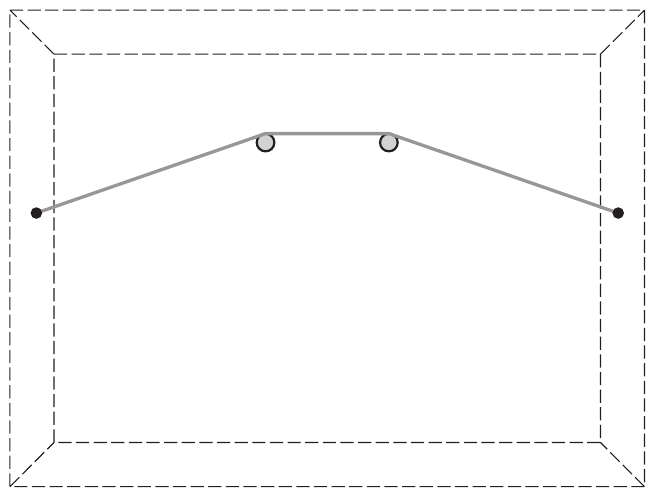
\includegraphics[scale=0.5]{pics/kartina1}
\caption{Эта картина останется висеть если выскочит один гвоздь.}
\end{figure}

\subsection*{Дефективный кодовый замок}

Кодовый замок имеет три крутильных диска, каждый из которых пронумерован от 1 до 8.
У замка есть дефект, чтобы его открыть, достаточно правильно выставить только два числа.
Какое минимальное количество (трёхзначных) комбинаций вам нужно проверить, чтобы точно открыть замок?

\parit{Комментарий:}
Есть много способов проделать это с $64$ тестовыми комбинациями, например, вы можете перебрать все возможные варианты первых двух дисков, или вы можете проверить все комбинации, сумма значений которых кратна 8.
Однако каждая тройная комбинация охватывает $22$ возможных случая, а всего существует только $8^3 = 512$ возможных комбинаций, поэтому в теории вам может удалиться сделать всего $\lceil 512/22 \rceil = 24$ тестовые комбинации.
Значит истина где-то между $24$ и $64$, вопрос где?

\subsection*{Альтернативные кости}

Можете ли вы создать две разные игральные кости так, чтобы их суммы вели себя так же, как пара обычных костей?
То есть должно быть два способа выбросить 3, шесть способов выбросить 7, один способ выбросить 12 и так далее. Каждая кость должна иметь шесть граней, и на каждой грани должно быть указано положительное целое число.

\subsection*{Совпадение монет}

Сонни и Шер играют в следующую игру.
В каждом раунде бросается честная монета.
Перед бросанием монеты Сонни и Шер одновременно объявляют свои предположения о результате броска монеты.
Они выигрывают раунд, если оба угадали правильно.
Цель --- максимизировать долю выигранных раундов, когда игра идет в течение многих раундов.

Пока что ответ очевиден --- 50\%: Сонни и Шер договариваются о последовательности предположений (например, они решают всегда говорить «орел»).
Очевидно они не могут добиться лучшего.

Однако перед началом игры игрокам сообщается, что прямо перед первым броском Шер получит результаты всех бросков монеты заранее!
Теперь у нее есть возможность обсудить стратегию с Сонни, но как только она получит информацию о броске монеты, дальнейшей возможности передачи информации не будет.
Возожно ли дотянуть долю выигрышей скажем до 70\%?

\subsection*{Имена в коробках}

Имена 100 заключенных помещают в 100 деревянных коробок, по одному имени в коробке;
коробки расставляются в комнате на столе.
Поочередно заключенных проводят в комнату;
каждый разрешается заглянуть не более чем в 50 коробок,
затем он должен покинуть комнату, оставив её в точно том же состоянии как раньше,
дальнейшее общение с другими невозможно.

У заключенных есть возможности спланировать свою стратегию заранее, и им это понадобится --- если хотя бы один заключенный не найдет свое собственное имя, то казнят всех.
Найдите стратегию, вероятность успеха которой превысит 30\%.

Комментарий: Если каждый заключенный откроет случайный набор из 50 коробок, то вероятность выжить составляет незавидные $(\tfrac12)^{100}\approx 0{,}0000000000000000000000000000008$.
Но они могли бы поступить и хуже --- если все откроют в одни и те же 50 коробок, то их шансы упадут до нуля. Но если тридцать процентов кажутся недостижимыми, то да --- вы правильно поняли задачу!
